%!TEX root = ../SciVis.tex

 Stream tubes are similar to streamlines, they display the paths of particles in a typically three-dimensional vector field as cylindrical tubes whose cross-section size can vary to encode additional parameters.
 
 To use this technique, we must first have a three-dimensional vector field,
 time-dependent simulation, if we consider time as the third (z) dimension. 
 
 should give you a three-dimensional 'data cube'. 
 
 holds raw simulation value, thus allows us to compute the scalar or vector field on the fly -> greater felxibility
 
 every simulation step -> add timeslice
 
 buffer[time][type][idx] , with idx being the index of the sample point implemented as 
 deque<vector<vector<fftw_floats> > > >
a deque  because it allows to easily push and pop data at both end. 
allows us to create a circular buffer without much effort
   
  
  
  
 
 
 
 
 
 \begin{figure}[htbp]
 \centering
 \begin{minipage}[t]{0.48\textwidth}
 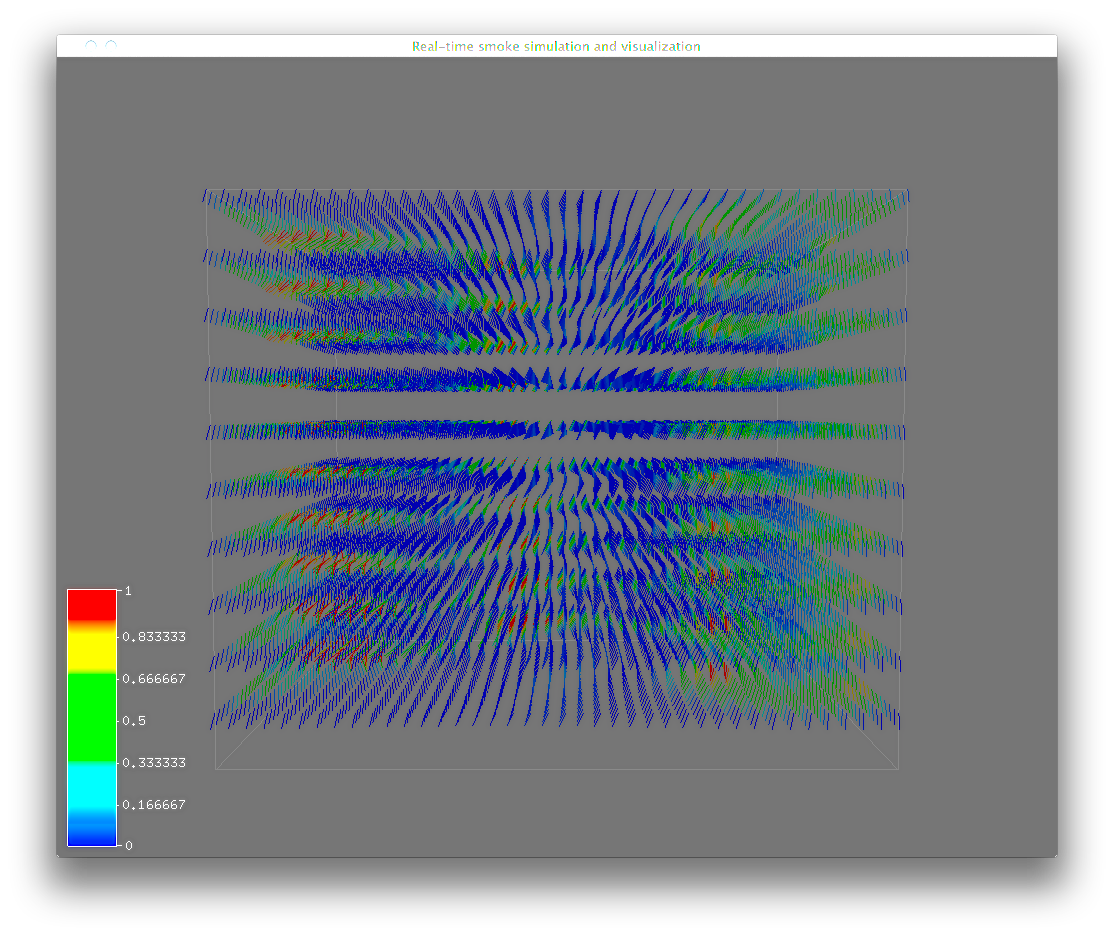
\includegraphics[height=3in]{figures/streamtubes/30datacube_bottom.png}
 \caption{Hedgehog visualization of the time-dependent velocity vector field. The individual time-slices are clearly visible if viewed from below.}
 \label{fig:datacube_bottom}
 \end{minipage}\hspace{.04\textwidth}%
 \begin{minipage}[t]{0.48\textwidth}
 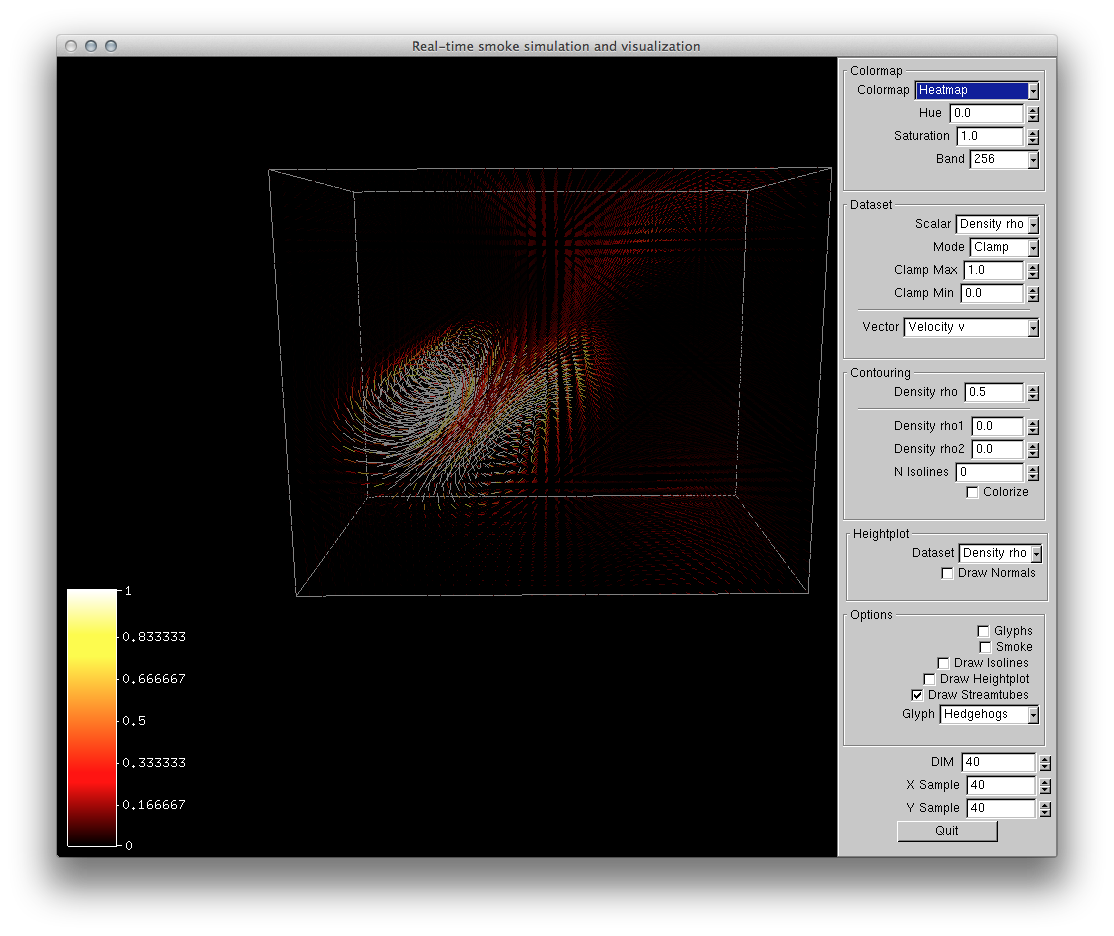
\includegraphics[height=3in]{figures/streamtubes/31datacube_front.png}
 \caption{Frontal view of the the time-dependent velocity vector field. Occlusion is a problem as the individual vectors/timeslices cannot be easily perceived.}
 \label{fig:}
 \end{minipage}
 \end{figure}
 
 
 place (and remove) seed points in the 3D volume.
 control the (x,y,z) position of a seed point by means of sliders. 
 allow users to click in some point in the window. 
 
 
 accomodate three dimensions instead of two.
 
 triliniear interpolation
    
    
pushed on 2D-vector that contains the actual pixel values of the streampoints + the scalar value at that point




  
  construct a stream tube geometry around it. 
  asubsequent step is to use a circle sampled as a closed polyline with n points, user-controlled

   For each sample point pi along a streamline, construct such a cross-section. The cross-section should be orthogonal to the current polyline segment pi, pi+1.

  
\begin{lstlisting}[language=C,caption={Cross-section in 3D reference frame}]
glBegin(GL_QUAD_STRIP);
  for (int i = 0; i <= 360; i = i + (360 / n)) {
    float theta = i * (M_PI / 180);
    float theta2 = (i + 1)*(M_PI / 180);
    
    float normal[3] = {};
    float vz[3] = {
        (cos(theta) * r) - (cos(theta) * rn),
        (sin(theta) * r)-(sin(theta) * rn),
         10 
    };
    float vx[3] = {
        (cos(theta) * r) - (cos(theta2) * r),
        (sin(theta) * r)-(sin(theta2) * r),
        0
    };
    normalize3(vz);
    normalize3(vx);
    crossproduct(vz, vx, normal);

    setColor(points[sp][3], TEXTURE);
    glNormal3f(normal[0], normal[1], normal[2]);
    glVertex3f(cos(theta) * r, sin(theta) * r, 0);

    setColor(points[sp + 1][3], TEXTURE);
    glNormal3f(normal[0], normal[1], normal[2]);
    glVertex3f(cos(theta) * rn, sin(theta) * rn, 15);

    setColor(points[sp][3], TEXTURE);
    glNormal3f(normal[0], normal[1], normal[2]);
    glVertex3f(cos(theta2) * r, sin(theta2) * r, 0);

    setColor(points[sp + 1][3], TEXTURE);
    glNormal3f(normal[0], normal[1], normal[2]);
    glVertex3f(cos(theta2) * rn, sin(theta2) * rn, 15);
  }
glEnd();
\end{lstlisting}  
  
 
 
 how to exactly place the cross-section? 
 
 a full reference frame in 3D, placed at each streamline point, which indicates the exact position and orientation of the cross-section. 
 
 get direction, local and up vector
 rotation matrix
 gets 'swept' along it


 \begin{lstlisting}[language=C, caption={Rotation and translation matrix to move cross-section along the streamtube.}]
 GLfloat R[16] = {
     local[0]     , local[1]     , local[2]     , 0,
     up[0]        , up[1]        , up[2]        , 0,
     target[0]    , target[1]    , target[2]    , 0,
     points[sp][0], points[sp][1], points[sp][2], 1
 };
 glMultMatrixf(R);
 \end{lstlisting}
 
 shading and coloring of the stream tubes: use either flat or Gouraud shading, and either a constant color,
 
 just use the colormapping functionalities from step 2. 
 the scalar field can be selected in the user interface
 a color map which shows one of the scalar fields along the streamline, such as velocity vector magnitude |v| or density rho.


(diameter) of the streamtubes. 
linearly scaled to show one of the scalar field values in the simulation, such as velocity vector magnitude |v| or density rho. 
all fields
affected by the radius of the next seed points



\begin{figure}[htbp]
\centering
\begin{minipage}[t]{0.48\textwidth}
        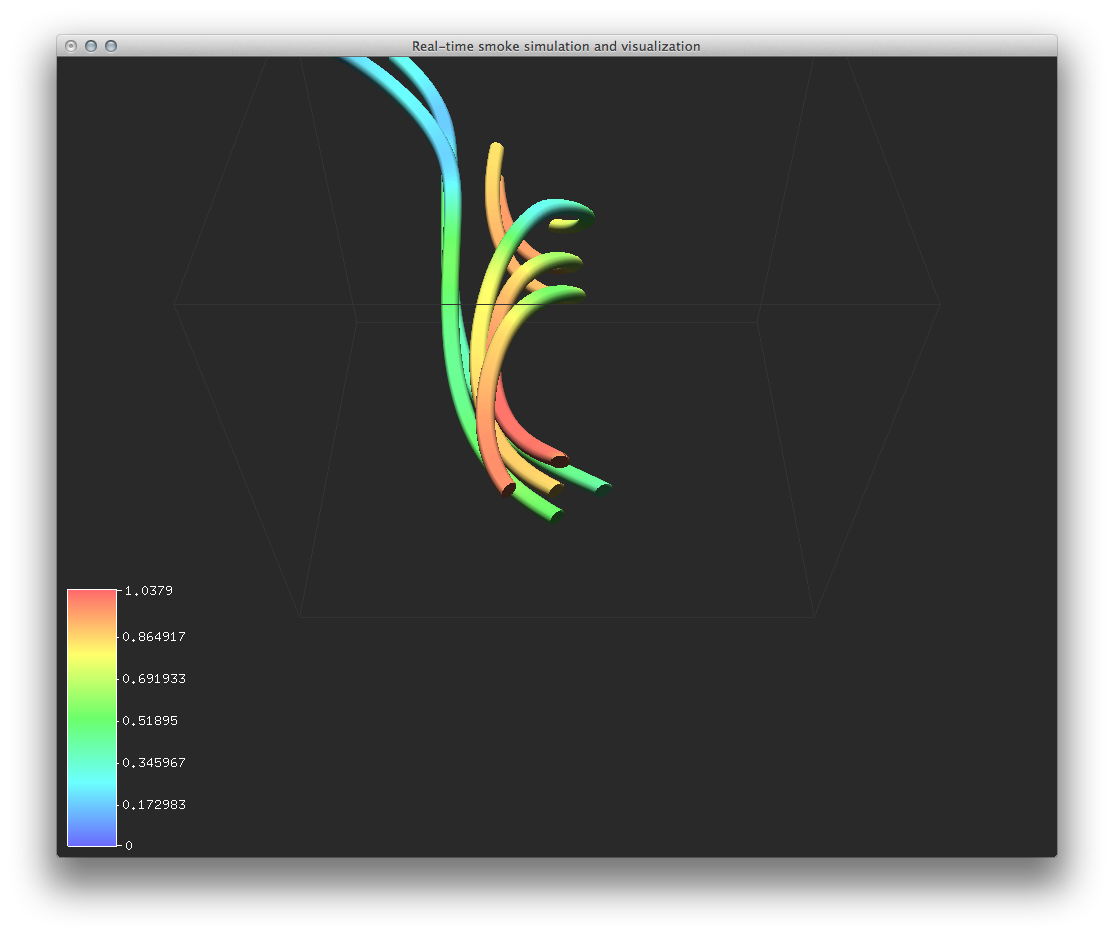
\includegraphics[height=3in]{figures/streamtubes/10tubes.png}
\caption{Combination of streamtubes and colormapping. Both techniques show the velocity. The seedpoints are centered in middle of the dataset.}
\label{fig:}
\end{minipage}\hspace{.04\textwidth}%
\begin{minipage}[t]{0.48\textwidth}
    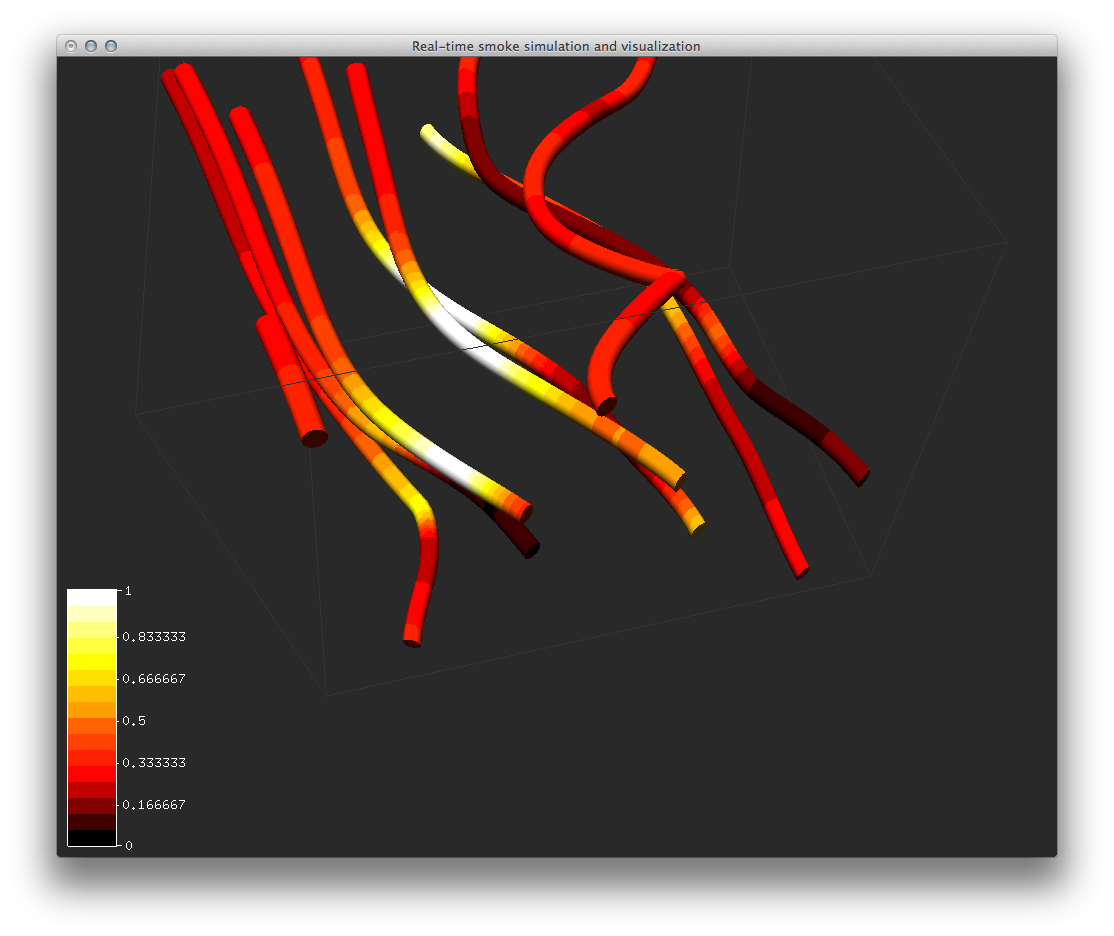
\includegraphics[height=3in]{figures/streamtubes/21banding_velodensity.png}
    \caption{Visualization of the velocity as streamtubes and density as heat colormap with a reduced number of colors. The banding effect makes the integration steps visible.}
    \label{fig:}
\end{minipage}
\end{figure}    

\begin{figure}[htbp]
\centering
\begin{minipage}[t]{0.48\textwidth}
        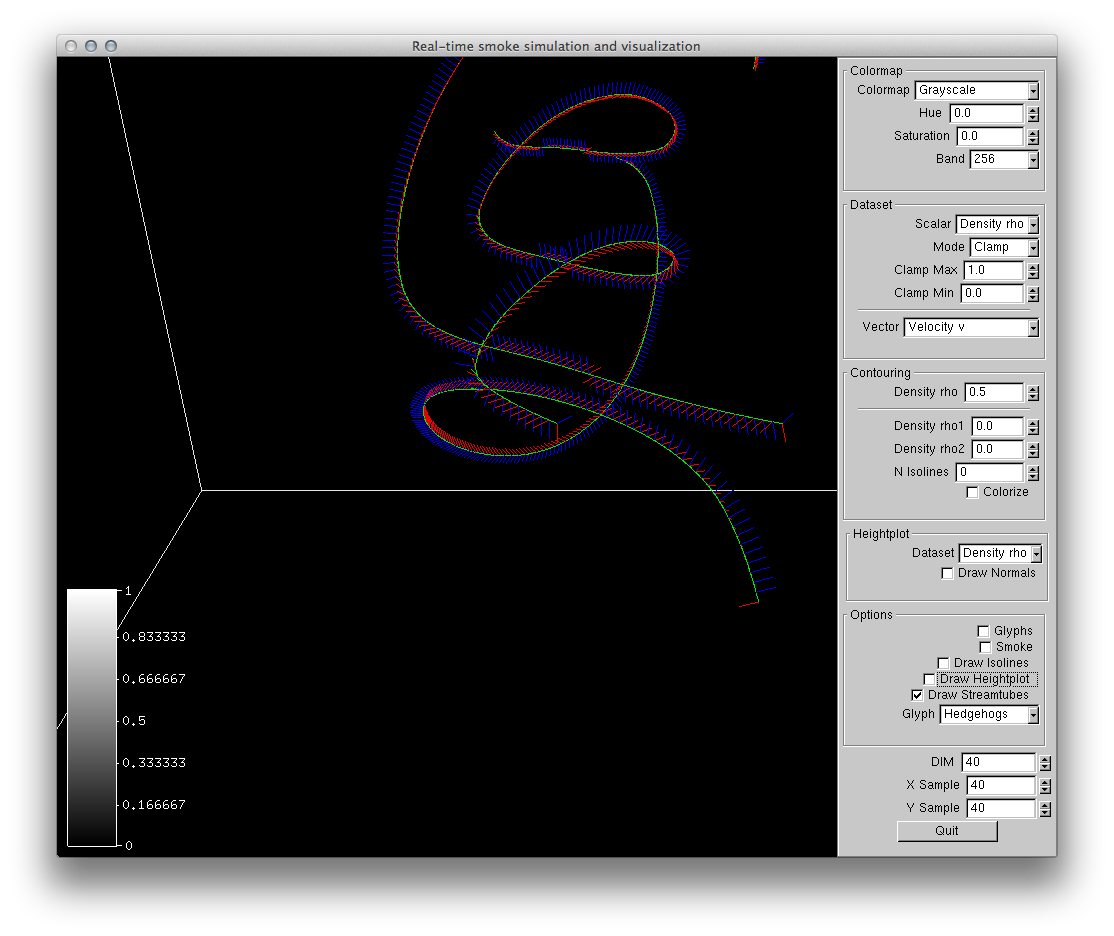
\includegraphics[height=3in]{figures/streamtubes/uvp.png}
\caption{Scaled orientation vectors. The green vector is tangent to the streamline, while the red and blue are perpendicular to the streamline.}
\label{fig:}
\end{minipage}\hspace{.04\textwidth}%
\begin{minipage}[t]{0.48\textwidth}
               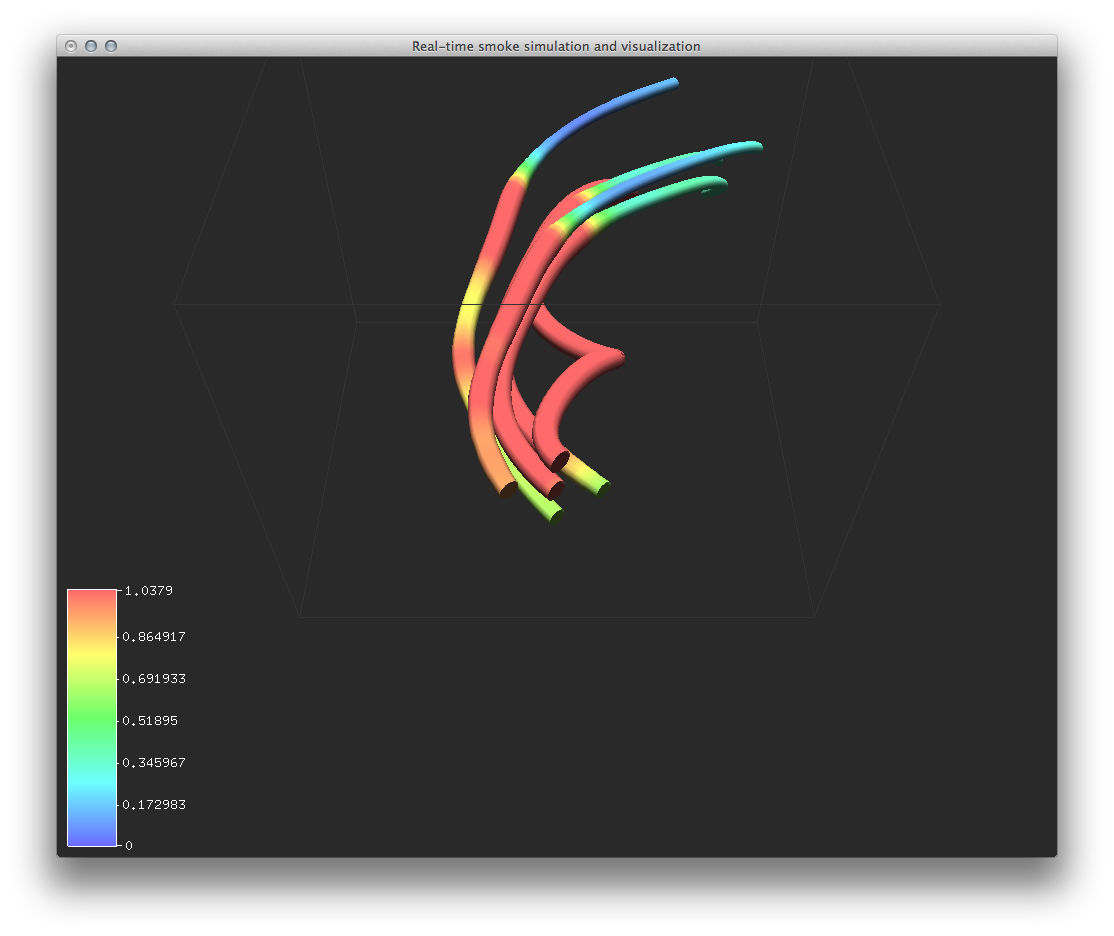
\includegraphics[height=3in]{figures/streamtubes/11thickTubes.png} 
    \caption{The diameter of the tube is linearly scaled based on a scalar value.}
    \label{fig:}
\end{minipage}
\end{figure}



\begin{figure}[htbp]
\centering
\begin{minipage}[t]{0.48\textwidth}
        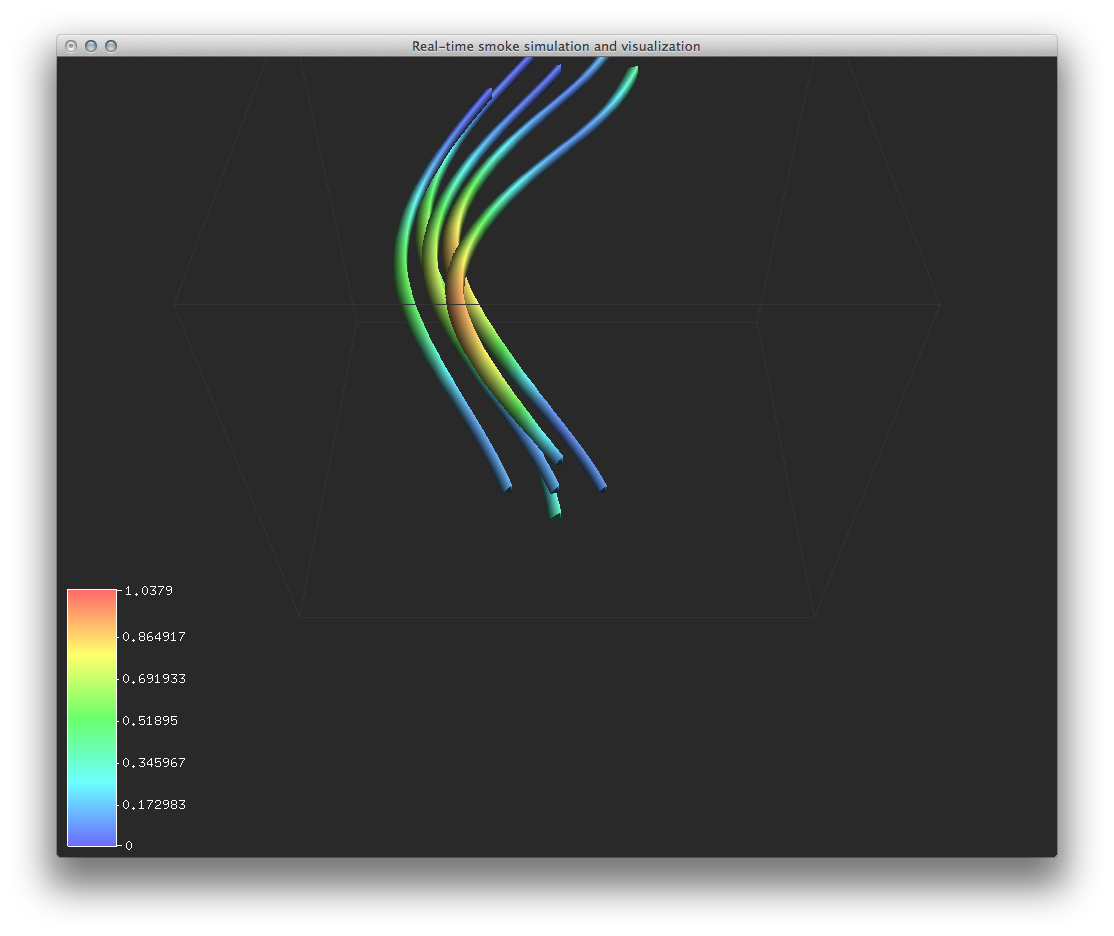
\includegraphics[height=3in]{figures/streamtubes/40threeSegments.png}
\caption{Triangular Tube geometry. The number of segments of the cross-sections can be adjusted dynamically.}
\label{fig:}
\end{minipage}\hspace{.04\textwidth}%
\begin{minipage}[t]{0.48\textwidth}
        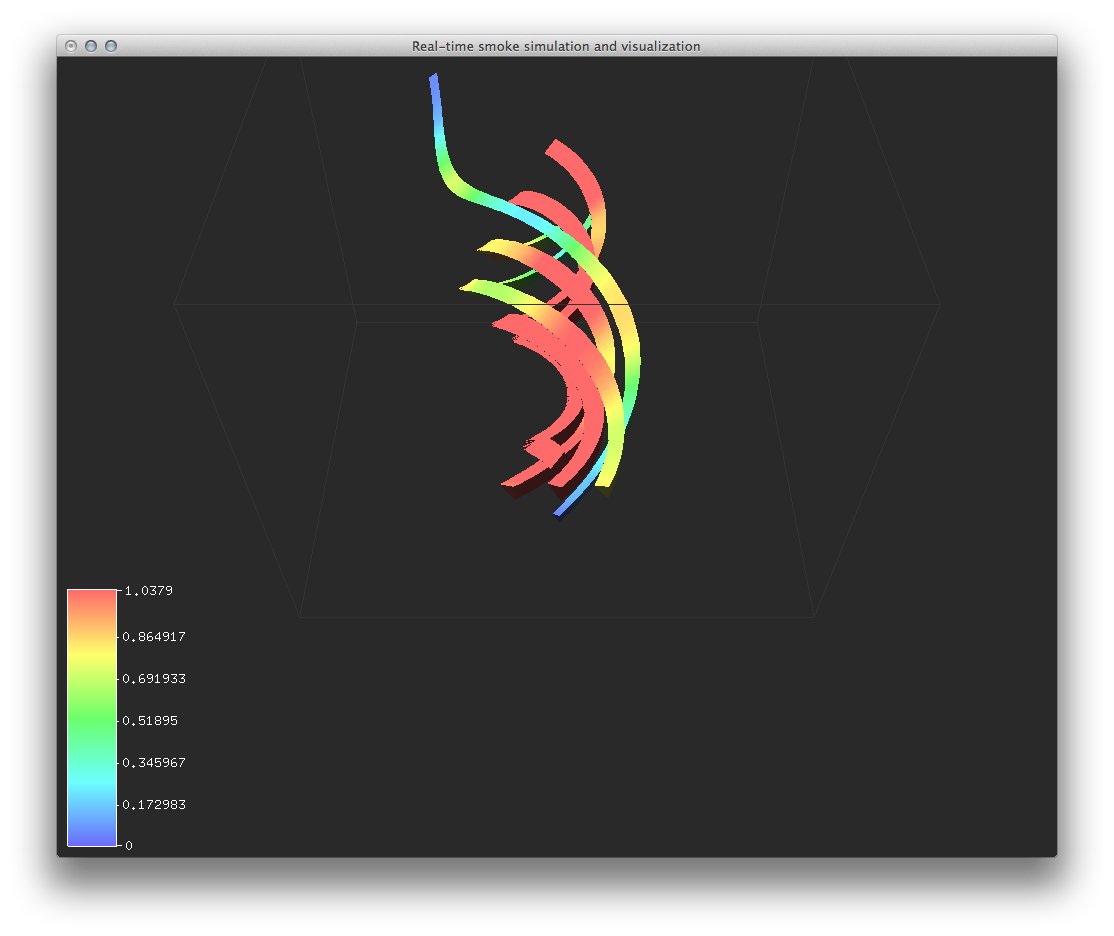
\includegraphics[height=3in]{figures/streamtubes/41flatshading.png}
    \caption{Flat shading accentuate the sharp-edges of the cross-section}
    \label{fig:}
\end{minipage}
\end{figure}

